\section{Expérience D2} \label{expD2}
  \subsection{Objectif}
    En partant de la seconde architecture de \cite{Cleeremans_2007}, 
    comprendre de quelles manières un réseau de neurone connexionniste peut, à partir de ses propres paris
    sur son résultat, améliorer son comportement.
  
  
  \subsection{Architecture}
    \paragraph{Description}
      Un premier réseau de perceptron multicouche apprend à discrétiser des chiffres représentés
      par 256 (16x16) neurones d'entrées. Il est composé d'une couche cachée de 100 neurones.
      
      Un second réseau de perceptron multicouche apprend à suivre une \textbf{intuition}
      représentant la ``distance'' entre l'indice du neurone gagnant le winner-take-all et l'indice
      du neurone ayant la bonne réponse.
      
      L'apprentissage du second réseau, n'affecte pas les poids entre la couche d'entrée et la 
      couche cachée du premier réseau.
    \paragraph{Schéma}
      \begin{center}
	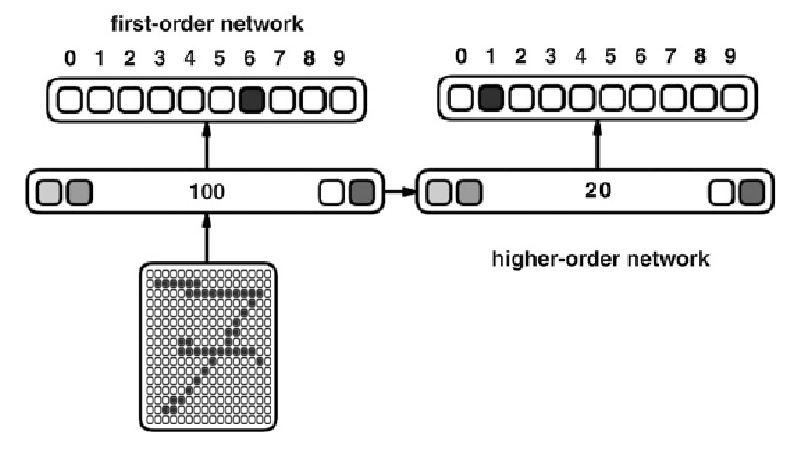
\includegraphics[width=220px]{data/expD2/schema.png}
      \end{center}
      
    \paragraph{Paramètres}
      \begin{center}
	\begin{tabular}{lr}
	  \begin{minipage}{230px}
	    \begin{itemize}
	      \item momentum : 0.5 sur le premier réseau
	      \item momentum : 0. sur le second réseau
	      \item taux d'apprentissage : 0.15 sur les 2 réseaux
	      \item \textbf{1600 formes} de chiffres différents présentées (shuffle) \cite{Handwritten_256}
	      \item apprentissage 50 (formes) x 300 (époques)
	      \item utilisation de biais
	      
	    \end{itemize}
	  \end{minipage}
	  &
	  \begin{minipage}{230px}
	    \begin{itemize}
	      \item poids initialisés sur [-1 ; 1] pour le premier réseau
	      \item poids initialisés sur [-0.25 ; 0.25] pour le second réseau
	      \item taux d'apprentissage constant
	      \item entrées valent 0 ou 1
	      \item sigmoïde à température 1
	    \end{itemize}
	  \end{minipage}
	\end{tabular}
      \end{center}

  
  \newpage
  \subsection{Résultats}
    \paragraph{Principaux}
      Analyse des performances
      \begin{center}
	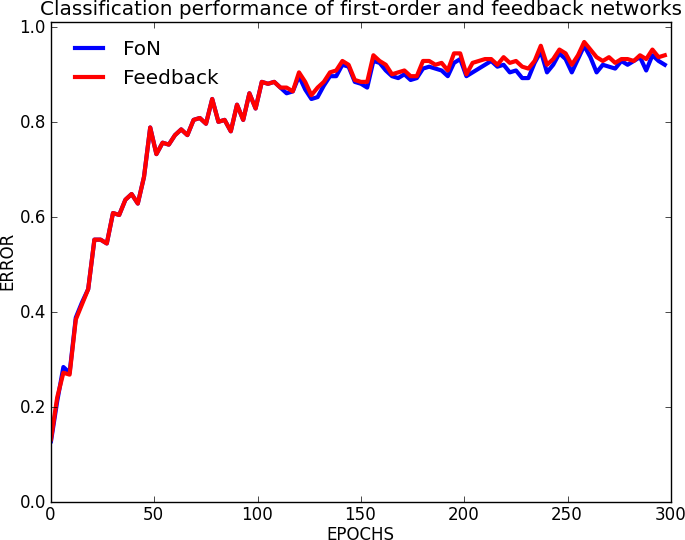
\includegraphics[width=250px]{data/expD2/perff.png}
      \end{center}
      \subparagraph{Notes}
	\begin{itemize}
	  \item la performance de classification représente le taux de bonnes réponses (winner-take-all) pour les 50 formes présentées sur une époque
	\end{itemize}
      \subparagraph{Conclusion}
	\begin{itemize}
	  \item l'architecture n'arrive qu'à une très faible augmentation de performance
	\end{itemize}
    \paragraph{Secondaires}
      Analyse des performances sous-jacentes
      \begin{center}
	\begin{tabular}{lr}
	  \hspace*{-1cm}
	  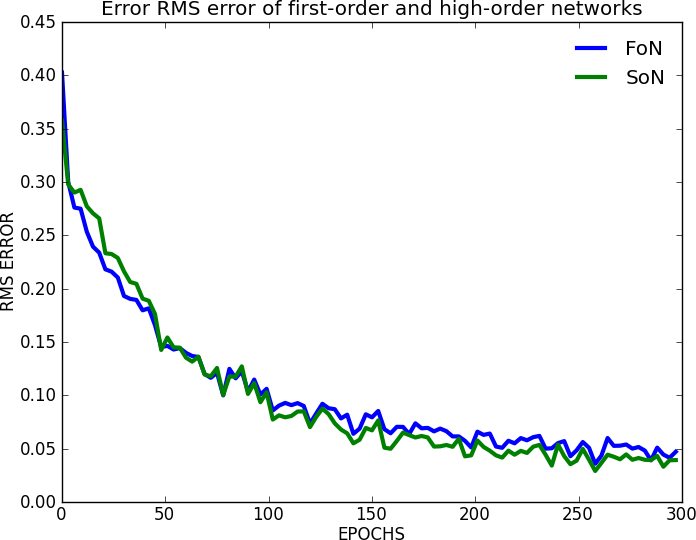
\includegraphics[width=250px]{data/expD2/rms.png}
	  &
	  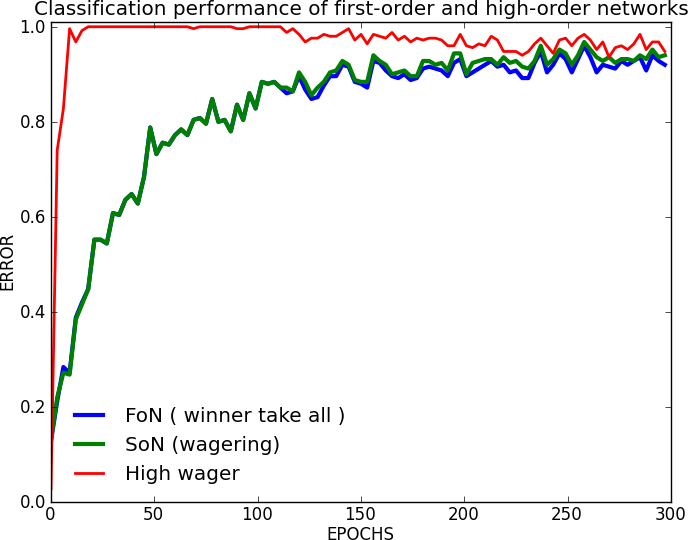
\includegraphics[width=250px]{data/expD2/perf.png} 
	\end{tabular}
      \end{center} 
      \subparagraph{Notes}
	\begin{itemize}
	  \item la courbe rouge représentent le taux de paris hauts (ie. premier neurone activé) du second réseau
	  \item la performance de classification représente le taux de bonnes réponses (winner-take-all) pour les 50 formes présentées sur une époque
	  \item formule utilisée pour RMS (cf. Formules~\nameref{rms})
	\end{itemize}
      \subparagraph{Conclusion}
	Cette fois-ci les performances du second réseau sont bien plus mitigées. N'ayant plus seulement 2 sorties mais 10, 
	il ne dépasse que de peu le premier réseau.


  \subsection{Conclusion}
  L'augmentation de performance est moindre, à cause d'une tâche plus ardue pour le second neurone.
  
  
  Avant de fermer ce chemin, il faudrait pousser un peu plus les recherches au niveau des paramètres choisis pour les réseaux.
  

  \newpage 
  \subsection{Formules}
    \paragraph{RMS} \label{rms}
  Pour une époque $e$ :
  \begin{center}
    \begin{large}
    $ rms_{e} = \sqrt{ \frac{1}{n} \sum \limits_{i=1}^{n} 
    ( o_{i,e} - d_{i} )^2 } $
    \end{large}
  $ with \left\lbrace \begin{array}{lll} n : number\ of\ neurons\ on\ the\ output\ 
  layer\\o_{i,e} : value\ obtained\ for\ the\ i^{th}\ neuron\ at\ the\ e^{th}\ epoch\\d_{i} : 
  value\ desired \ for\ the\ i^{th}\ neuron\end{array} \right.$
  \end{center}
    
    \paragraph{Descente de gradient} \cite{Touzet_1992} \\
  Construction de l'erreur : 
    \begin{center}
      $y_{i} = f'(a_i) \times ( d_i - x_i ) \ si\ i\ neurone\ de\ sortie $ \\
      $y_{i} = f'(a_i) \times \sum \limits_{k} ( w_{ki} \times y_k )\ si\ i\ neurone\ cache $
    \end{center}
  Mise à jour des poids :
    \begin{center}
      $w_{ij}(t+1) = w_{ij}(t) + learning\_rate \times y_{i} \times x_j + momentum \times 
      (w_{ij}(t) - w_{ij}(t-1) )$
    \end{center}
  Variables : 
    \begin{center}
      $\left\lbrace \begin{array}{lll} 
	f : fonction\ sigmoide \\
	x_i : valeur\ du\ neurone\ i\\
	d_i : valeur\ desire pour\ le\ neurone\ i\\
	a_i : somme\ pondere\ des\ poids\ du\ neurone\ i
      \end{array} \right.$
    \end{center}
    
\bibliographystyle{../pre-rapport/apalike}
\bibliography{../pre-rapport/biblio}
